\documentclass[conference]{IEEEtran}
\usepackage{cite}
\usepackage{amsmath,amssymb}
\usepackage{graphicx}
\usepackage{booktabs}
\usepackage{array}
\usepackage{url}
\begin{document}
\title{Regularised Environmental and Fire-History Models for Daily Hotspot Occurrence in California}
\author{\IEEEauthorblockN{Ayush Singh}\IEEEauthorblockA{Department of Computational Intelligence\\SRM Institute of Science and Technology\\Kattankulathur, India\\as5790@srmist.edu.in}
\and\IEEEauthorblockN{Sarvadnya Kulkarni}\IEEEauthorblockA{Department of Computational Intelligence\\SRM Institute of Science and Technology\\Kattankulathur, India\\ss9878@srmist.edu.in}}
\maketitle
\begin{abstract}
Daily satellite fire activity depends on environmental conditions and the persistence of recent burning. We propose a regularised environmental--history modelling framework that combines nonlinear additive responses with tree-based predictions through validation-selected convex weights. The framework includes matched directional constraints, joint optimisation of a multiplicative environmental index, and a separate probability-calibration stage. Observed ERA5 weather, MODIS vegetation, SRTM terrain and VIIRS detections cover 2021--2024 on a $0.25^\circ$ California grid. Models are trained on 2021--2022, selected and calibrated on disjoint subsets of 2023, and evaluated on 2024 after these choices are frozen. The selected convex ensemble achieves AUC-ROC 0.847, average precision 0.2564 and Brier score 0.01807 on 232,168 complete test cell-days, of which 4,959 are positive. Its highest-scored decile captures 58.0\% of positives with precision 12.40\%. Comparisons with persistence, seasonal climatology and simpler environmental models distinguish ranking skill from the contribution of model complexity. The target is observed hotspot occurrence, and same-day reanalysis does not establish advance ignition forecasting skill.
\end{abstract}
\begin{IEEEkeywords}
Wildfire, hotspot occurrence, additive models, regularisation, ensemble learning, calibration.
\end{IEEEkeywords}

\section{Introduction}
A satellite hotspot indicates observed thermal activity at an overpass, not necessarily the start of a new fire. A large fire may remain detectable for days, while clouds, smoke and acquisition timing can hide ongoing activity~\cite{viirs}. This distinction changes how a daily fire model should be designed and evaluated. Recent detections can be informative even without environmental predictors, so persistence is an essential comparator rather than a nuisance to be ignored.

Weather, vegetation and terrain provide additional context. Heat and atmospheric dryness influence fuel conditions, vegetation indices describe aspects of fuel and canopy state, and wind and slope can affect fire behaviour. Fire radiative power (FRP) characterises observed combustion activity~\cite{wooster}. These relationships motivate candidate features, but they do not uniquely determine a statistical formula. In particular, a positive physical association need not produce a positive coefficient after conditioning on correlated variables, and a product of normalized drivers can impose restrictive interactions.

We propose a framework that retains a transparent environmental representation while allowing nonlinear responses and complementary tree predictions. The additive component uses cubic splines with both ridge and coefficient-difference penalties. A convex combination of additive and tree probabilities supplies the ensemble component; its weights are selected on validation data. The mathematical restrictions are tested through matched linear fits and a jointly tuned multiplicative alternative. Calibration is selected separately so that a ranking gain is not mistaken for accurate probabilities.

The contribution is a reproducible regional method and evaluation, rather than a claim to a new universal physical law. Three design choices are central: penalties are made explicit when comparing directional constraints; skewed fire histories are transformed before modelling; and a later year is reserved for testing after model and calibration selection. We use an observed four-year dataset, report all family winners and include strong persistence and climatology baselines. The experiment asks whether the proposed modelling procedure improves the ranking and probability estimation of hotspot cell-days at this spatial and temporal scale.

\section{Study Area and Observations}
\subsection{Sources, labels and spatial support}
The study covers California from 1 January 2021 through 31 December 2024. The working domain spans $32$--$42^\circ$N and $124$--$114^\circ$W. We retain the 660 centres of a $0.25^\circ$ grid that lie within the US Census California boundary. The mask applies to centres rather than clipping cell polygons; retained coastal and border cells can therefore include water or land outside the state.

ERA5 hourly single-level reanalysis provides 2-m temperature and dewpoint, both 10-m wind components, and volumetric water in the 0--7 cm soil layer~\cite{era5}. All 48 monthly regional weather files are included in the data archive. They were subset from the public Earthmover ERA5 mirror~\cite{earthmover}. NASA FIRMS standard-processing VIIRS S-NPP detections provide labels and fire histories~\cite{firms,viirs}. We retain type-0 vegetation detections with nominal or high confidence. A cell-day is positive if it contains at least one retained detection; multiple observations in the same cell-day do not create additional positive labels.

MOD13A1.061 supplies 500-m, 16-day NDVI and near- and mid-infrared reflectances (bands 2 and 7)~\cite{modis}. All four years use the same product and nearest native pixel sampling through the Microsoft Planetary Computer COG archive~\cite{planetary}. Raw sampled values, quality flags and unsigned source URLs are retained. SRTM elevation supplies static terrain slope, averaged within each analysis cell~\cite{srtm}. A cell-centre vegetation sample and a cell-mean slope have different spatial support; neither resolves within-cell fuel or topographic heterogeneity.

\subsection{Alignment, quality control and histories}
Daily weather is aggregated in UTC. Inputs are maximum temperature, maximum wind-speed magnitude, mean surface soil water and humidity calculated from temperature and dewpoint at the hour of maximum temperature. The humidity field is not the minimum of the 24 hourly humidity values. ERA5 is sampled at the nearest source point, with lower-coordinate resolution of exact distance ties. MODIS canopy moisture is represented by $(\mathrm{NIR}-\mathrm{MIR})/(\mathrm{NIR}+\mathrm{MIR})$ after valid-range checks. The NDWI label here denotes this spectral proxy, not a direct measurement of leaf water content.

MODIS reliability flags 0 and 1 are retained; cloud, snow and fill observations are excluded. A composite becomes available only after its window ends, including the shortened final window at the year boundary. Valid completed observations are carried forward for at most 48 days. Rows still missing a required driver are omitted. This rule avoids backward interpolation but does not simulate actual operational publication latency. Missingness can also change the evaluated population, particularly where quality failures are systematic.

For each cell and day $t$, FRP and count histories use only days $t-1$ through $t-7$, with lag weight $0.5^k$. The current day's detections never enter its history features. Histories are zero-initialised at the start of 2021; later year boundaries retain the preceding days normally. Daily labels are constructed before dropping incomplete feature rows, so a missing vegetation observation does not break the fire-history sequence. This supports retrospective monitoring of continuing activity; it does not resolve whether an observed hotspot belongs to a new incident.

\subsection{Training, selection and test populations}
Scaling limits are fitted on 2021--2022 only and frozen. Continuous drivers are min--max scaled and later values clipped to $[0,1]$; any subsequent standardisation is also fitted only on training rows. Table~\ref{tab:data} reports complete observations after quality control. Test metrics use these rows, not the number of raw detections or all possible grid-days.

\begin{table}[!t]\centering\footnotesize
\caption{Model-ready observations after quality control. Training: 2021--2022; selection/calibration: 2023; test: 2024.}\label{tab:data}
\begin{tabular}{rrrr}\toprule
Year & Cell-days & Positives & Rate (\%)\\\midrule
2021 & 230,463 & 6,633 & 2.88 \\
2022 & 216,925 & 4,539 & 2.09 \\
2023 & 219,909 & 5,246 & 2.39 \\
2024 & 232,168 & 4,959 & 2.14 \\
\bottomrule\end{tabular}\end{table}

Within each month of 2023, days 1--14 form the model-selection set and days 22 through month-end form the calibration set. Days 15--21 are unused in those decisions. This preserves seasonal coverage in both subsets. It does not eliminate dependence across month boundaries, and the subsets are not independent seasonal trials. All candidate parameters and calibration choices are frozen before model performance is calculated on 2024. Previous development on earlier years informed the search design; the newly acquired 2024 labels did not select its settings.

\section{Proposed Modelling Framework}
\subsection{Environmental representation and matched linear fits}
The nine drivers are scaled temperature, NDVI, canopy dryness $1-\widetilde{\mathrm{NDWI}}$, atmospheric dryness $1-\widetilde{\mathrm{RH}}$, soil dryness $1-\widetilde{\mathrm{SM}}$, wind, slope, prior FRP and prior count. The last two can be transformed as $g(h)=\log(1+1000h)$, where $h$ is the normalized history. The fixed constant changes the feature response scale; it is not a physical conversion of FRP units. It expands differences among small histories while compressing extreme activity.

Matched linear fits minimise
\begin{equation}
\begin{aligned}
 L(w,b)&=\frac1n\sum_{i=1}^{n}\left[\log(1+e^{z_i})-y_i z_i\right]\\
 &\quad+\frac{\|w\|_2^2}{2Cn},\qquad z_i=b+x_i^\top w.
\end{aligned}
\end{equation}
The intercept is unpenalised. The constrained version adds $w_j\geq0$, while the free version uses the same objective without bounds. Both are fitted with the same solver and tolerances. Standardized raw and log-history representations are crossed with $C\in\{0.1,1,10\}$ and both sign conditions, yielding 12 fits. This design separates the sign restriction from a change in penalty or feature scale.

\subsection{Smooth additive component}
The proposed interpretable component represents the logit as
\begin{equation}
 z_i=b+\sum_{j=1}^{9}\sum_{k}\theta_{jk}B_{jk}(x_{ij}),
 \qquad p_i=\frac{1}{1+e^{-z_i}}.
\end{equation}
Cubic B-spline bases use training-quantile knots, with three, five or seven knots per driver. Their columns are standardized on training data. The objective adds both ridge regularisation and a second-difference penalty~\cite{eilers}:
\begin{equation}
\begin{aligned}
 L_{\rm smooth}&=L_{\rm Bernoulli}+\frac{\|w\|_2^2}{2Cn}\\
 &\quad+\frac{\lambda}{2}\sum_j\|D_2\theta_j\|_2^2.
\end{aligned}
\end{equation}
Here $w$ denotes coefficients of standardized basis columns, and $\theta$ denotes coefficients on the original basis scale. The omitted final basis coefficient is anchored at zero; the intercept absorbs a common level shift. The implementation therefore divides by the training basis scales before applying $D_2$. The difference penalty discourages abrupt changes between neighbouring coefficients. With nonuniform knots it is a discrete roughness penalty, not an exact integrated squared-derivative penalty.

We cross the three knot counts with $C\in\{0.1,1,10\}$ and $\lambda\in\{0,0.01,0.1\}$, giving 27 candidates. The zero-roughness cases retain ridge regularisation and serve as a controlled comparison. No monotonicity restriction is imposed on the spline terms. Their shapes describe conditional fitted associations and should not be interpreted as intervention effects.

\subsection{Joint multiplicative formulation}
A complementary physical index tests whether a compact product can represent the same inputs:
\begin{align}
 D_i&=a_1x_{{\rm canopy},i}+a_2x_{{\rm air},i}+a_3x_{{\rm soil},i},\\
 R_i&=\left[(\epsilon+\tilde T_i)(\epsilon+\widetilde{\rm NDVI}_i)
 (\epsilon+D_i)\right]^q\notag\\
 &\quad\cdot(1+b_U\tilde U_i+b_\theta\tilde\theta_i)\notag\\
 &\quad+\eta\left[r\,g_H(\widetilde{\rm FRP}_i)+(1-r)g_H(\widetilde{\rm Count}_i)\right].
\end{align}
Dryness weights lie on the nonnegative unit simplex. Wind and slope weights range from 0 to 2; $r$ lies in $[0,1]$. The sampled offsets are $\{0,0.03,0.1,0.3,0.7\}$, history scales $\{0.1,0.3,1,3,10\}$, and powers $\{0.5,1,2\}$. Ninety-six seeded parameter configurations include one fixed reference. Each is paired with raw history $g_H(h)=h$ and compressed history $g_H(h)=\log(1+1000h)/\log(1001)$, giving 192 joint-index candidates. The latter retains a unit-range history factor while allowing the same compression used in the additive and tree components. Each receives a training-fitted scalar logistic mapping with $C=100$ after standardisation.

Joint search allows the relative contributions of dryness, spread and history to adjust together. Offsets reduce zero-gating when a normalized factor approaches its training minimum, while $q$ changes the environmental response shape. These are statistical design choices. The index is not the Canadian Fire Weather Index, and its normalized zeros are not physical combustion thresholds. The search is finite and does not prove a globally optimal equation.

\subsection{Tree components and convex combination}
Random Forest, XGBoost and LightGBM provide complementary nonlinear components~\cite{breiman,xgboost,lightgbm}. Their 36 refinement configurations vary tree depth or leaf count, estimator count, leaf-size restrictions and ridge penalties. Nine matched comparisons use the original distribution, inverse-frequency weighting or training-only SMOTE followed by undersampling at a common configuration within each tree family. SMOTE raises the minority/majority ratio to 0.10 and undersampling to 0.30; these fits do not simultaneously apply class weights. All tree components use log-compressed histories.

XGBoost crosses depths 3, 5 and 7, estimator counts 200, 500 and 800, and ridge values 1 and 10. LightGBM crosses leaf counts 15, 31 and 63, estimator counts 300 and 600, and ridge values 1 and 10. Both use learning rate 0.04; XGBoost uses minimum child weight 10, row fraction 0.8 and feature fraction 0.9, while LightGBM uses minimum child size 40. Random Forest uses 300 trees, depths 8, 12 or unlimited, and minimum leaf sizes 5 or 20. The matched class-handling comparisons use 300 trees, depth 5 for Random Forest/XGBoost, 31 leaves for LightGBM, boosted ridge 5 and Random Forest minimum leaf size 10. Seeds are fixed at 42.

The complete search contains 276 fitted configurations. Within the additive, Random Forest, XGBoost and LightGBM families, the candidate with highest selection average precision (AP) is retained. We then form
\begin{equation}
 p_{\rm ens}(x)=\sum_{m=1}^{4}\pi_m p_m(x),\qquad
 \pi_m\geq0,\quad\sum_m\pi_m=1.
\end{equation}
The ensemble search includes 128 seeded simplex draws and the four vertices. Vertices allow selection to retain a single model when averaging is unhelpful. We select by pooled AP on the designated 2023 rows, breaking ties with AUC-ROC. The final model is the best declared candidate or blend under this rule. Quarterly selection metrics are retained as diagnostics; they do not replace the declared selection criterion. Component selection and blend search use the same validation subset, so their uncertainty and possible validation overfitting remain part of the method's limitations.

\subsection{Probability calibration}
Probability mapping follows model selection. Days 22--25 of each 2023 month fit identity, sigmoid-on-logit and isotonic alternatives; the remaining calibration days select the mapping with lowest Brier score. The selected mapping is refitted on all calibration rows. A sigmoid with nonpositive slope is excluded. Isotonic mapping may introduce ties, so both raw and mapped ranking metrics are retained. No 2024 labels enter model training, weight selection or calibration.

\section{Evaluation Design}
We compare with fixed weather-only logistic regression, a same-cell prior-day/prior-week persistence model, and cell-rate plus annual sine/cosine climatology. The climatology uses a smoothed training-cell event rate; each training row's own label is excluded from its rate. A constant forecast equal to the training prevalence supplies the probability reference. All nonconstant baselines receive the same calibration-selection procedure as the candidate family winners.

Metrics are AUC-ROC, AP, Brier score and capture within the highest-scored 10\% of complete cell-days. AP's no-skill reference is test prevalence. The inspection budget is rounded upward and score ties use stable row order; capture can therefore depend on ordering at a tied boundary. Brier skill is $1-B/B_{\rm const}$, where the constant uses the training event rate. Metrics measure different properties: global ranking, positive retrieval, probability accuracy and performance at one budget.

Paired circular moving-block bootstraps use block lengths 7 and 30 days and 300 replicates each. Consecutive days are sampled modulo the 366-day test year and truncated to a full year. All cell-days are retained via day multiplicities, with identical weights for every model; no negative-class subsampling is used. Percentile intervals describe paired AUC and AP differences. They condition on the fitted models and observed year, do not account for the full model-selection procedure, and do not establish transfer to other regions.

\section{Results}
\subsection{Held-out performance}
Selection chooses the convex ensemble with 2023 selection AP 0.2664. The chosen probability mapping is sigmoid. On 2024, its AUC is 0.847 and AP is 0.2564 against prevalence 0.0214. Table~\ref{tab:performance} reports all family winners and baselines on the identical complete test population. Bold type marks the validation-selected method. The highest test AP belongs to the convex ensemble (0.2564); the test ranking is reported without changing the selection rule.

\begin{table*}[!t]\centering\footnotesize
\caption{2023 selection and held-out 2024 test performance. Capture is recall at a 10\% row budget. Baselines have no comparable tuned selection score.}\label{tab:performance}
\begin{tabular}{lrrrrr}\toprule
Model & Selection AP & Test AUC & Test AP & Brier & Capture (\%)\\\midrule
Regularised linear logit & 0.2161 & 0.795 & 0.2090 & 0.01881 & 49.9 \\
Smooth additive logit & 0.2347 & 0.820 & 0.2298 & 0.01853 & 54.5 \\
Joint multiplicative index & 0.2216 & 0.756 & 0.2085 & 0.01859 & 51.3 \\
XGBoost & 0.2621 & 0.846 & 0.2552 & 0.01808 & 58.2 \\
LightGBM & 0.2609 & 0.846 & 0.2538 & 0.01811 & 58.0 \\
Random Forest & 0.2645 & 0.845 & 0.2534 & 0.01811 & 57.5 \\
\textbf{Convex ensemble} & 0.2664 & 0.847 & 0.2564 & 0.01807 & 58.0 \\
Hotspot persistence & --- & 0.742 & 0.1325 & 0.01900 & 55.5 \\
Cell and season climatology & --- & 0.753 & 0.0735 & 0.02036 & 35.2 \\
Weather-only logit & --- & 0.549 & 0.0228 & 0.02090 & 9.3 \\
Constant training rate & --- & 0.500 & 0.0214 & 0.02092 & --- \\
\bottomrule\end{tabular}\end{table*}

\begin{figure*}[!t]\centering
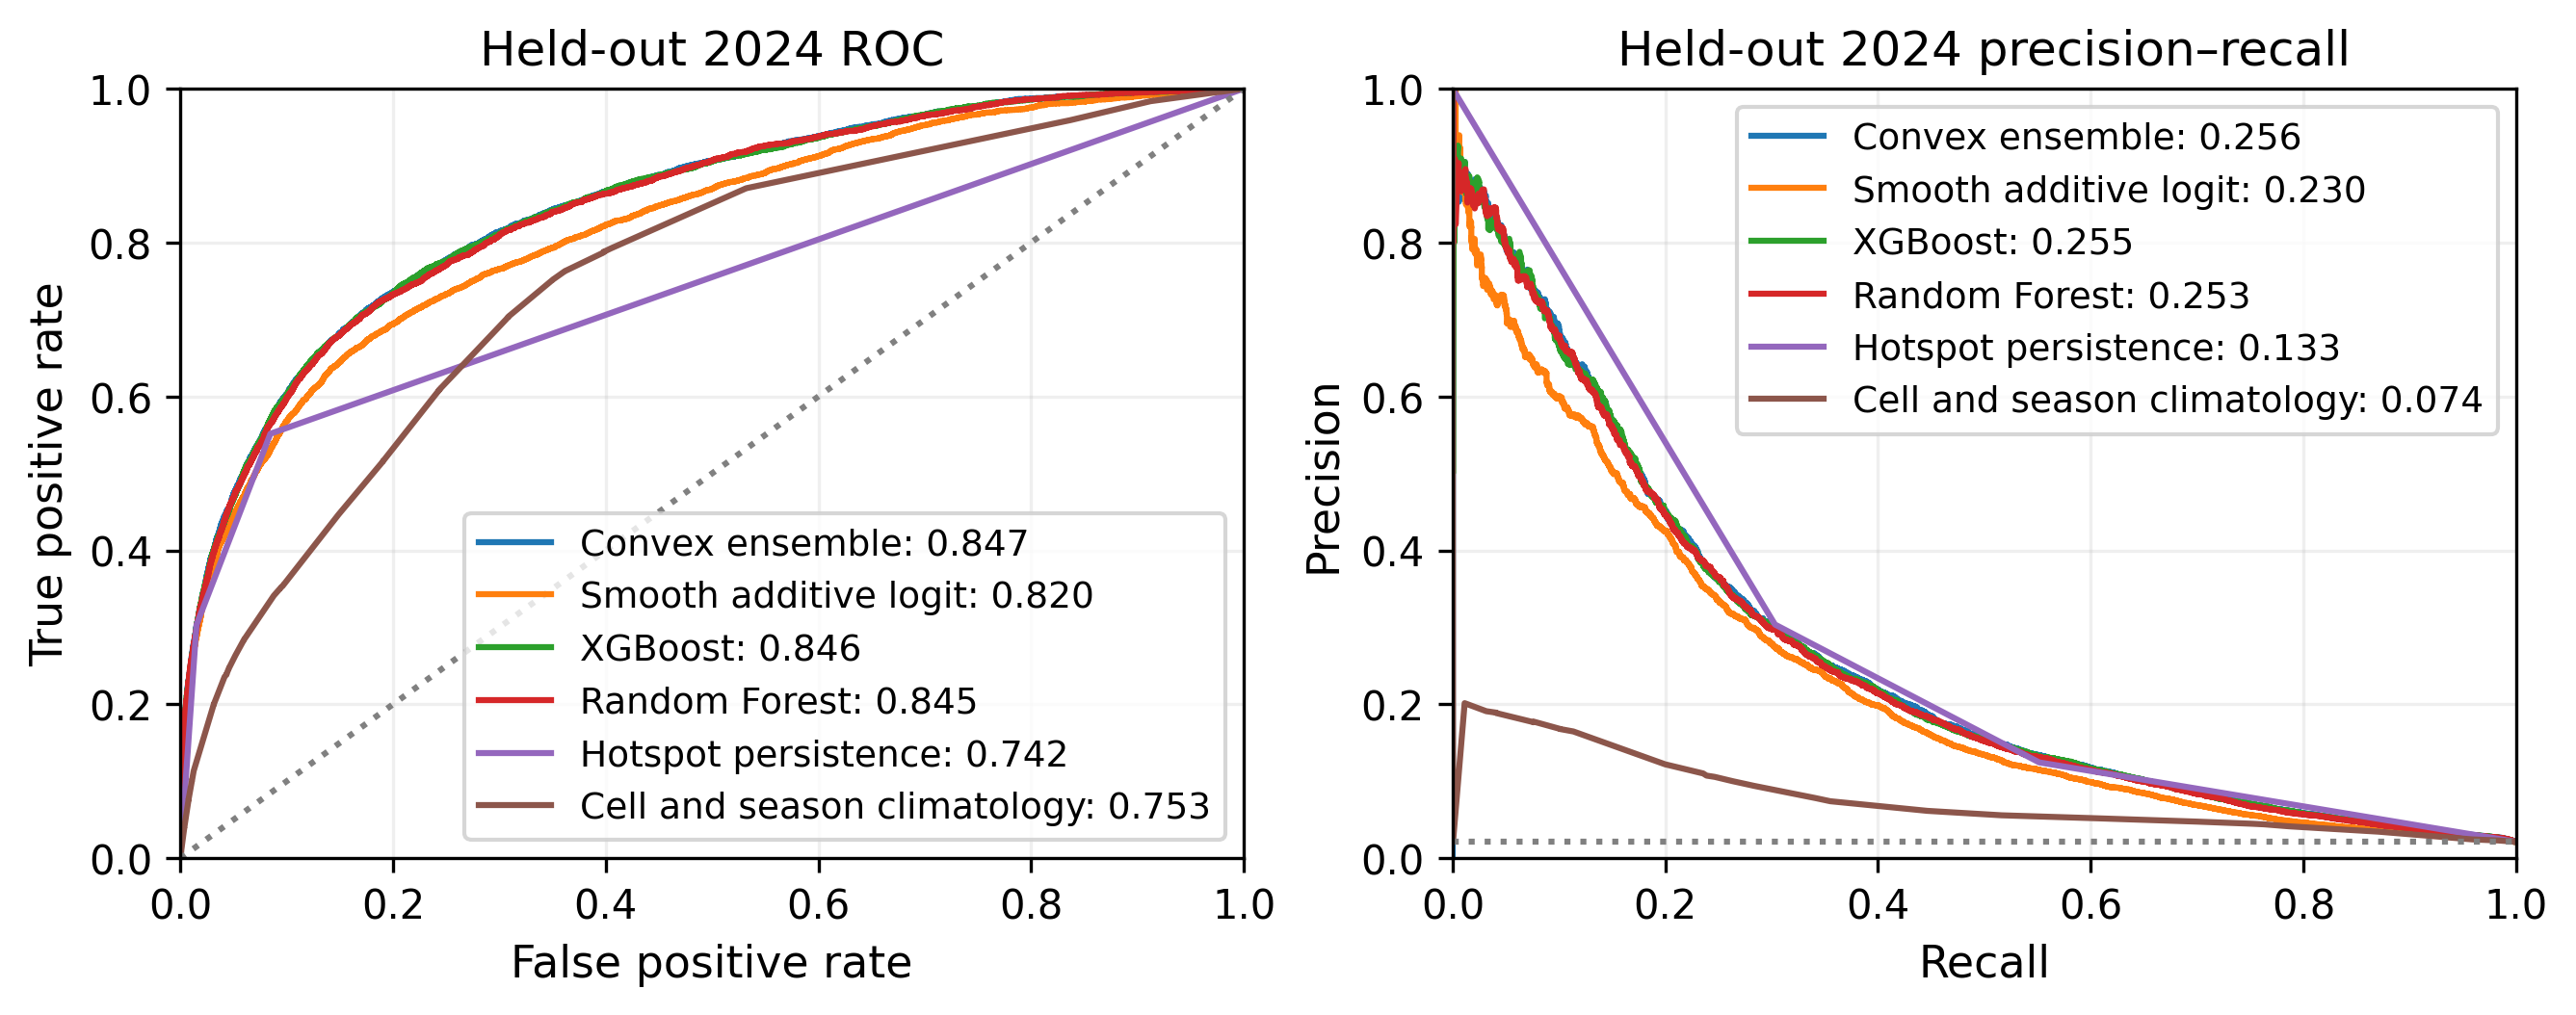
\includegraphics[width=.96\textwidth]{outputs/standalone/discrimination.png}
\caption{Held-out 2024 ROC and precision--recall curves from saved predictions. Legends give AUC and AP; the dotted precision line denotes test prevalence.}\label{fig:discrimination}
\end{figure*}

At the stated budget, 23,217 selected cell-days contain 2,878 positives. This corresponds to capture 58.0\% and precision 12.40\%. The count is not the number of separate fires detected: continued activity can contribute multiple positive days in the same cell. An operational interpretation would additionally require incident linkage, response costs and an inspection capacity chosen before deployment.

\subsection{Model structure and calibration}
Table~\ref{tab:intervals} places the small ensemble gains in context. At the 30-day block length, the AP interval against XGBoost includes zero, whereas those against Random Forest, LightGBM and the smooth additive model are positive. This supports a modest gain over some components, but not a clear advantage over XGBoost. The intervals condition on this fitted search and are not adjusted for multiple comparisons.

The selected smooth component uses 5 knots, $C=1$ and $\lambda=0$, achieving test AUC 0.820 and AP 0.2298. The jointly tuned multiplicative family scores AUC 0.756 and AP 0.2085. The selected convex weights are Smooth additive logit 0.028, Random Forest 0.511, XGBoost 0.283, LightGBM 0.179. These values describe the fitted method, rather than universal environmental importance. Full candidate settings and quarterly validation diagnostics are included with the code.

The best validation AP among ridge-only splines ($\lambda=0$) is 0.2347, compared with 0.2196 among positive-roughness candidates. Thus including a mathematically motivated penalty in the search does not itself establish a benefit. In the 96 paired index configurations, log-compressed history improves validation AP in 94 cases, with median paired change +0.0127. The best raw-history and compressed-history index scores are 0.0568 and 0.2216, respectively. These are validation comparisons used to understand the search, not additional independent test results.

\begin{figure*}[!t]\centering
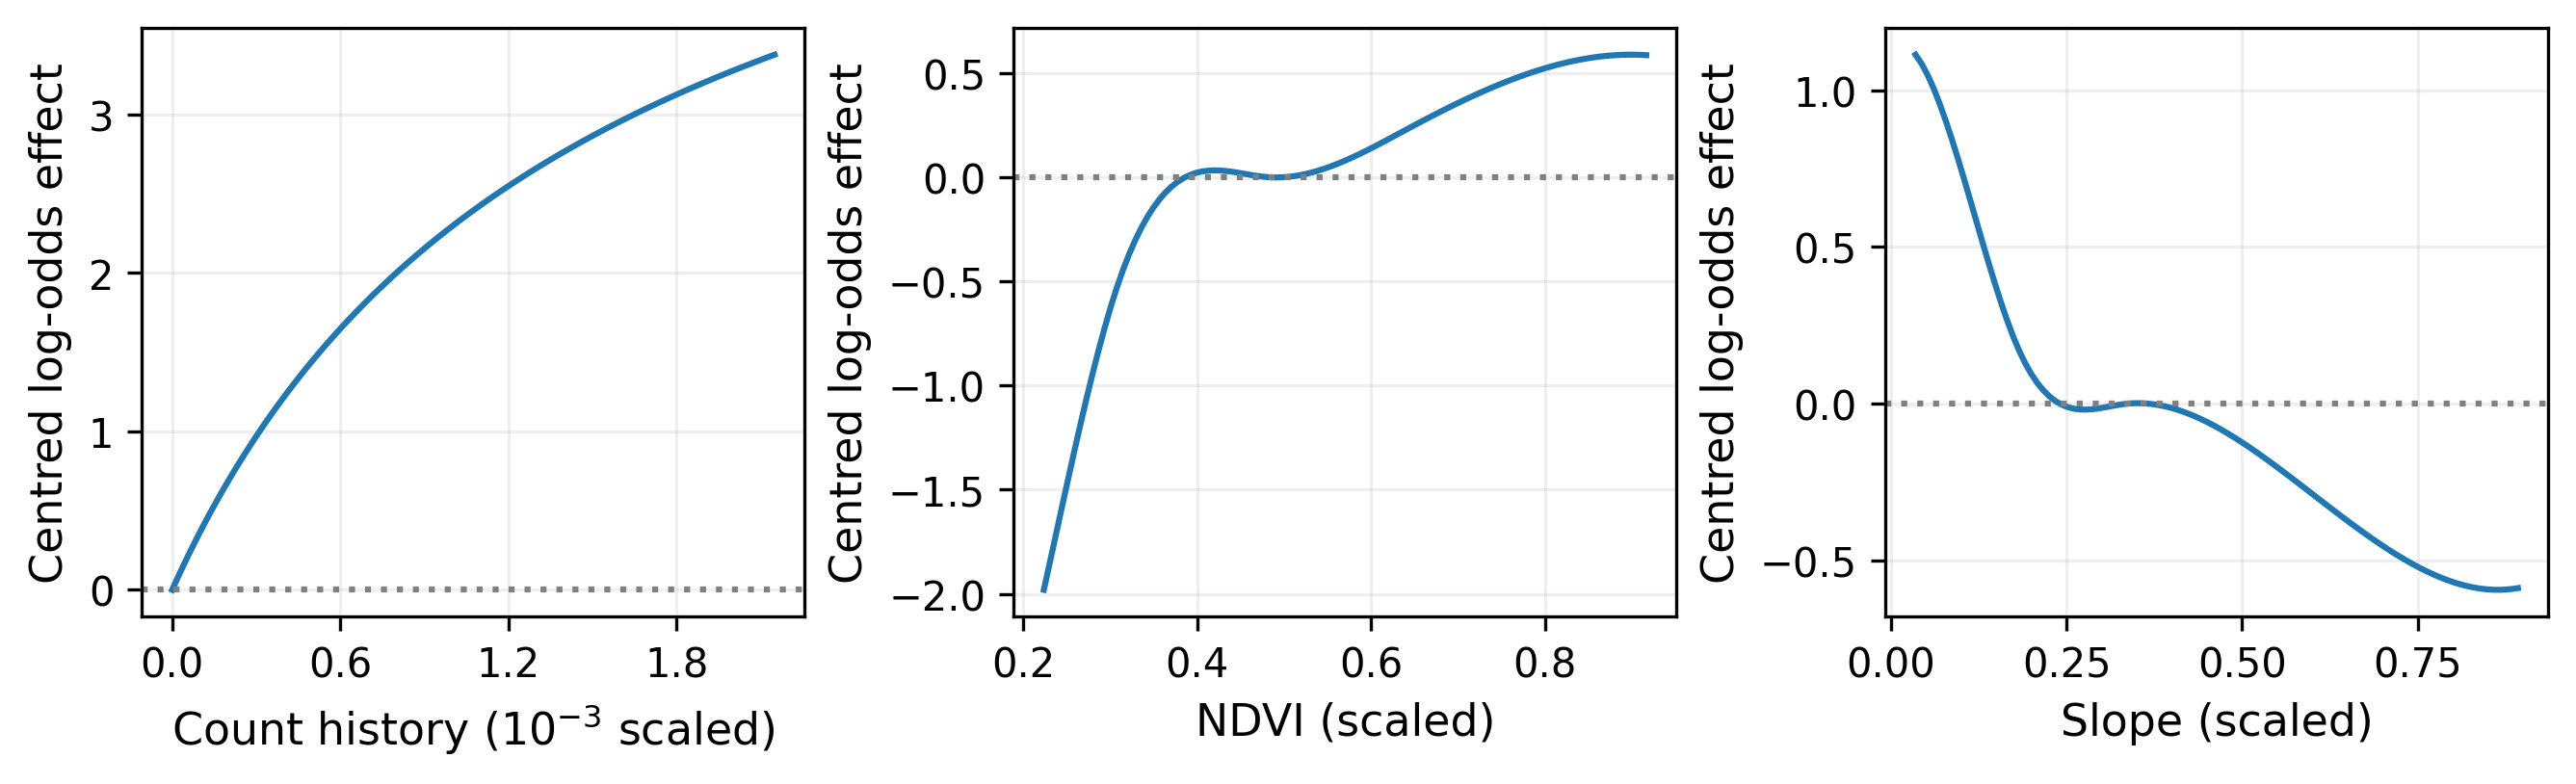
\includegraphics[width=.96\textwidth]{outputs/standalone/smooth_effects.png}
\caption{Three smooth terms with the largest fitted effect ranges between the training 1st and 99th percentiles. Other inputs are fixed at training medians; effects are centred there. Axes show training-scaled inputs. These are conditional model effects, not causal responses.}\label{fig:effects}
\end{figure*}

The selected model's mean probability is 0.0220, giving a mean-to-observed-rate ratio of 1.03. Its Brier score is 0.01807 and training-rate-reference Brier skill is 0.136. The maximum absolute observed--predicted gap among the ten equal-count bins is 0.0101. Equal-count reliability bins help describe the broad probability range but can conceal within-bin errors and a small extreme tail.

The raw and mapped selected-model Brier scores are 0.018035 and 0.018066, respectively. Calibration selected on 2023 therefore slightly worsens this 2024 score, despite bringing the overall mean probability closer to prevalence. We retain the frozen mapping; a post-test switch would bias evaluation.

\begin{figure}[!t]\centering
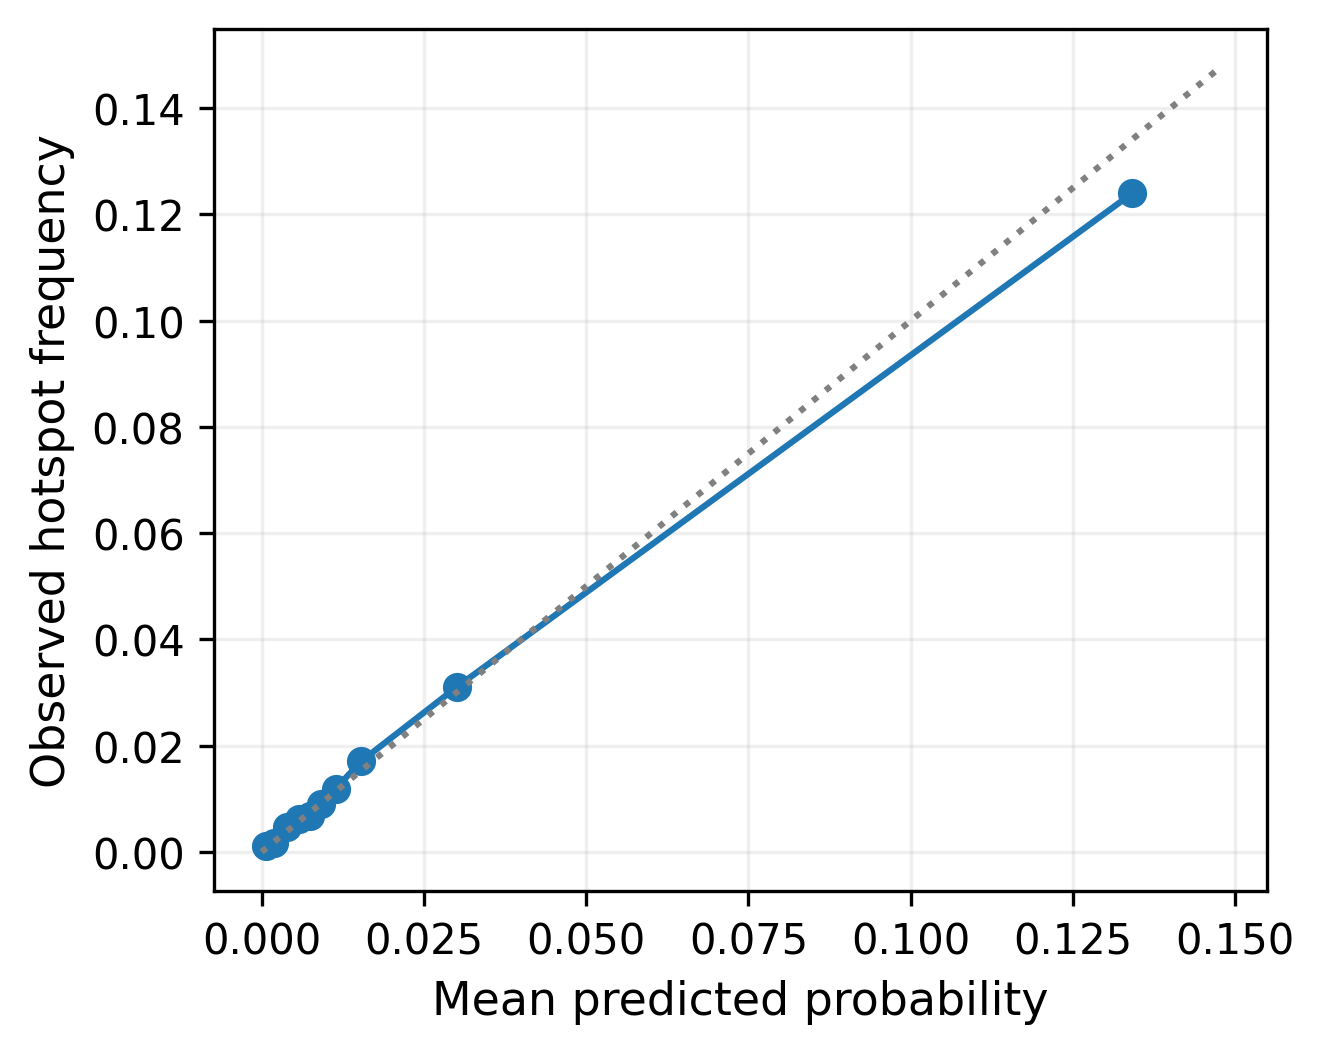
\includegraphics[width=.94\columnwidth]{outputs/standalone/reliability.png}
\caption{Final selected probabilities versus observed 2024 occurrence in ten equal-count bins. The dotted line represents exact calibration.}\label{fig:reliability}
\end{figure}

\begin{table*}[!t]\centering\footnotesize
\caption{Selected method minus comparator: paired 2024 AUC and AP differences with moving-day-block 95\% intervals.}\label{tab:intervals}
\begin{tabular}{rlrrrr}\toprule
Block days & Comparator & AUC difference & Interval & AP difference & Interval\\\midrule
7 & Smooth additive logit & +0.02693 & [+0.02112, +0.03256] & +0.02656 & [+0.01734, +0.03407] \\
7 & Random Forest & +0.00221 & [+0.00139, +0.00300] & +0.00297 & [+0.00154, +0.00442] \\
7 & XGBoost & +0.00086 & [+0.00009, +0.00158] & +0.00119 & [-0.00069, +0.00300] \\
7 & LightGBM & +0.00044 & [-0.00069, +0.00152] & +0.00255 & [+0.00015, +0.00495] \\
7 & Hotspot persistence & +0.10486 & [+0.09431, +0.11440] & +0.12386 & [+0.09775, +0.14753] \\
30 & Smooth additive logit & +0.02693 & [+0.01889, +0.03525] & +0.02656 & [+0.01557, +0.03621] \\
30 & Random Forest & +0.00221 & [+0.00108, +0.00314] & +0.00297 & [+0.00150, +0.00440] \\
30 & XGBoost & +0.00086 & [-0.00004, +0.00174] & +0.00119 & [-0.00064, +0.00307] \\
30 & LightGBM & +0.00044 & [-0.00055, +0.00169] & +0.00255 & [+0.00032, +0.00518] \\
30 & Hotspot persistence & +0.10486 & [+0.09458, +0.11627] & +0.12386 & [+0.08857, +0.15534] \\
\bottomrule\end{tabular}\end{table*}

\section{Discussion and Limitations}
The validation-selected blend places 97.2\% of its weight on tree components. Its performance should therefore not be attributed mainly to the smooth term or to a new physical law. Log-compressed history helps the joint index, but that family remains weaker than the selected ensemble on the held-out year. The zero-roughness spline wins its family search, providing no evidence here that the additional difference penalty improves retrieval.

Environmental effects remain associational. Terrain, vegetation, human activity and observation conditions are spatially correlated. A nonlinear slope or dryness term may absorb several unmeasured processes. The apparent contribution of recent fire history can reflect continuation of the same event, while coarse cells and cell-centre vegetation sampling mix heterogeneous conditions. Quality filtering and the 48-day vegetation-age limit also select which cell-days enter evaluation. Performance on omitted observations is unknown.

The experiment uses two training years and one test year in one region. Although 2024 was reserved from model scoring until all choices were frozen, one successful annual transfer cannot establish stability across fire regimes. The moving-block intervals preserve local episode structure more faithfully than independent-row resampling, but depend on the chosen block length and circular boundary assumption. They exclude uncertainty from alternative training years and the large validation search. Additional untouched years and spatial holdouts would provide stronger evidence.

Finally, all weather aggregates are same-day reanalysis. A prospective forecast would require weather available at issuance time and a lead-time-specific evaluation. A new-ignition target would require incident-linked or otherwise independently validated onset labels. The proposed method addresses retrospective daily hotspot occurrence; neither a high AUC nor good average calibration converts it into a validated operational ignition-warning system.

\section{Conclusion}
We present a regularised environmental--history framework for daily observed hotspot occurrence, with nonlinear additive terms, jointly tuned physical factors and validation-selected convex model combinations. Training on 2021--2022 and freezing selection and calibration on 2023 gives a held-out 2024 AUC of 0.847 and AP of 0.2564 for the selected convex ensemble. Its highest-scored decile captures 58.0\% of positive cell-days. The supplied source observations, complete candidate ledger, trained models and predictions make the comparison reproducible. The result supports evaluation of the proposed method at the stated regional scale while retaining clear limits on causal and prospective interpretation.

\section*{Acknowledgment}
The authors acknowledge Copernicus, NASA FIRMS and LP DAAC, Microsoft Planetary Computer, Earthmover, USGS and the US Census Bureau for source data and public access services.

\begin{thebibliography}{00}
\bibitem{viirs} W.~Schroeder, P.~Oliva, L.~Giglio, and I.~A.~Csiszar, ``The new VIIRS 375 m active fire detection data product,'' \emph{Remote Sensing of Environment}, vol.~143, pp.~85--96, 2014, doi:10.1016/j.rse.2013.12.008.
\bibitem{wooster} M.~J.~Wooster, G.~Roberts, G.~L.~W.~Perry, and Y.~J.~Kaufman, ``Retrieval of biomass combustion rates and totals from fire radiative power observations,'' \emph{Journal of Geophysical Research: Atmospheres}, vol.~110, D24311, 2005, doi:10.1029/2005JD006318.
\bibitem{era5} Copernicus Climate Change Service, ``ERA5 hourly data on single levels from 1940 to present,'' Climate Data Store, doi:10.24381/cds.adbb2d47.
\bibitem{earthmover} Earthmover, ``Icechunk ERA5: public reanalysis archive,'' Registry of Open Data on AWS, \url{https://registry.opendata.aws/earthmover-era5/}, accessed Nov.~2026.
\bibitem{firms} NASA FIRMS, ``VIIRS S-NPP 375 m active fire detections: Standard Processing,'' \url{https://firms.modaps.eosdis.nasa.gov/content/descriptions/FIRMS_VIIRS_Firehotspots.html}, accessed Nov.~2026.
\bibitem{modis} NASA LP DAAC, ``MODIS Vegetation Index User's Guide, Collection 6.1,'' \url{https://lpdaac.usgs.gov/documents/621/MOD13_User_Guide_V61.pdf}, accessed Nov.~2026.
\bibitem{planetary} Microsoft, ``MODIS Vegetation Indices 16-Day (500m), MOD13A1.061,'' Planetary Computer, \url{https://planetarycomputer.microsoft.com/dataset/modis-13A1-061}, accessed Nov.~2026.
\bibitem{srtm} NASA LP DAAC, ``SRTM Collection User Guide,'' \url{https://lpdaac.usgs.gov/documents/179/SRTM_User_Guide_V3.pdf}, accessed Nov.~2026.
\bibitem{eilers} P.~H.~C.~Eilers and B.~D.~Marx, ``Flexible smoothing with B-splines and penalties,'' \emph{Statistical Science}, vol.~11, no.~2, pp.~89--102, 1996, doi:10.1214/ss/1038425655.
\bibitem{breiman} L.~Breiman, ``Random forests,'' \emph{Machine Learning}, vol.~45, pp.~5--32, 2001, doi:10.1023/A:1010933404324.
\bibitem{xgboost} T.~Chen and C.~Guestrin, ``XGBoost: A scalable tree boosting system,'' in \emph{Proc. ACM SIGKDD}, 2016, pp.~785--794, doi:10.1145/2939672.2939785.
\bibitem{lightgbm} G.~Ke \emph{et al.}, ``LightGBM: A highly efficient gradient boosting decision tree,'' in \emph{Advances in Neural Information Processing Systems}, vol.~30, 2017.
\end{thebibliography}
\end{document}